%------------------------------------------------
% Request.tex
%
% This document build the incident frame
%------------------------------------------------
\section{Request Fulfillment}
\frame
{
\frametitle{Contenuti}
\tableofcontents[currentsection]
%\addtocounter{framenumber}{-1}
}

\subsection*{Input e Output}
\begin{frame}{Input e Output}
Input:
\begin{table}
\begin{tabular}{ l | c }
\textbf{Input} & \textbf{Da}\\
\hline
RFC & Utenti\\
\end{tabular}
\caption{input di processo}
\end{table}
Output:
\begin{table}
\begin{tabular}{ c | c }
\textbf{Output} & \textbf{Da}\\
\hline
Notifiche & Utenti\\
\end{tabular}
\caption{output di processo}
\end{table}
\end{frame}

\subsection*{Attività di processo}
\begin{frame}{Attività di processo}
\begin{figure}
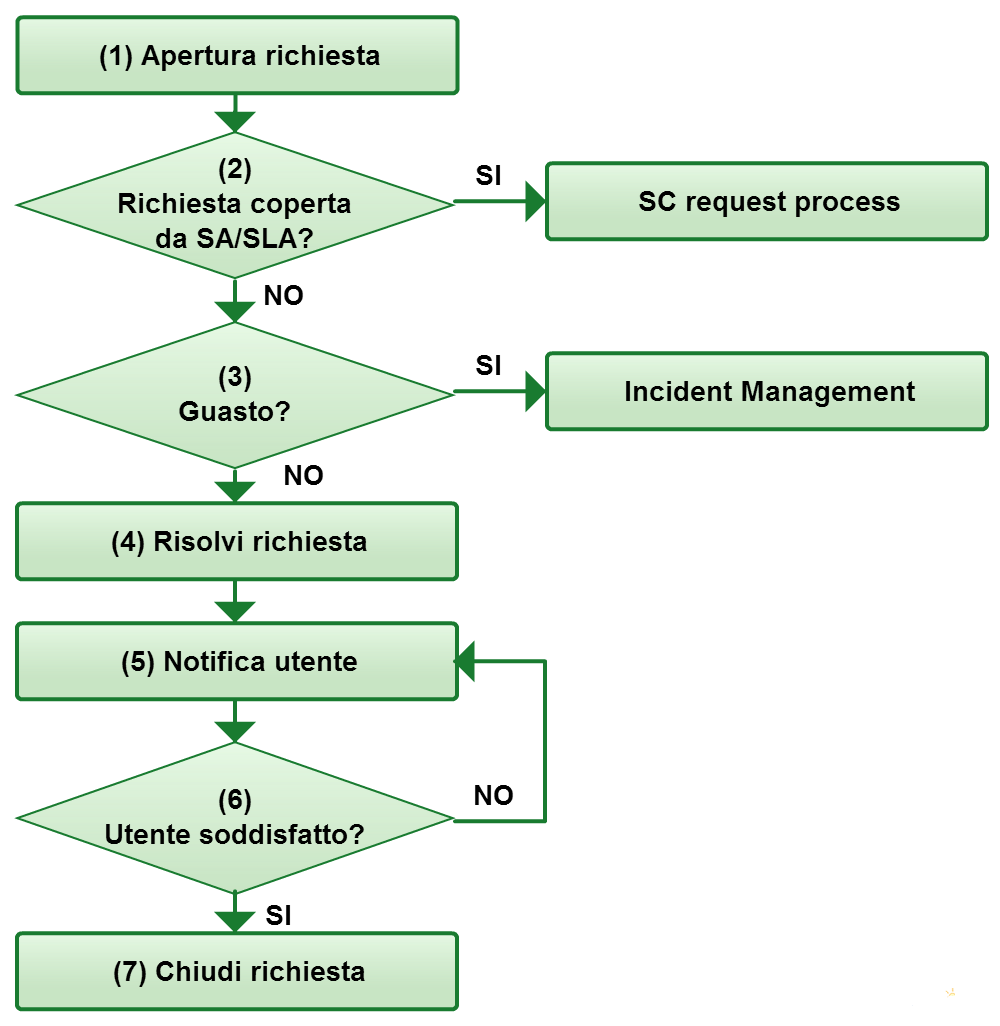
\includegraphics[scale=0.22]{Images/Request_fulfillment.png}
\end{figure}
\end{frame}